\begin{center}
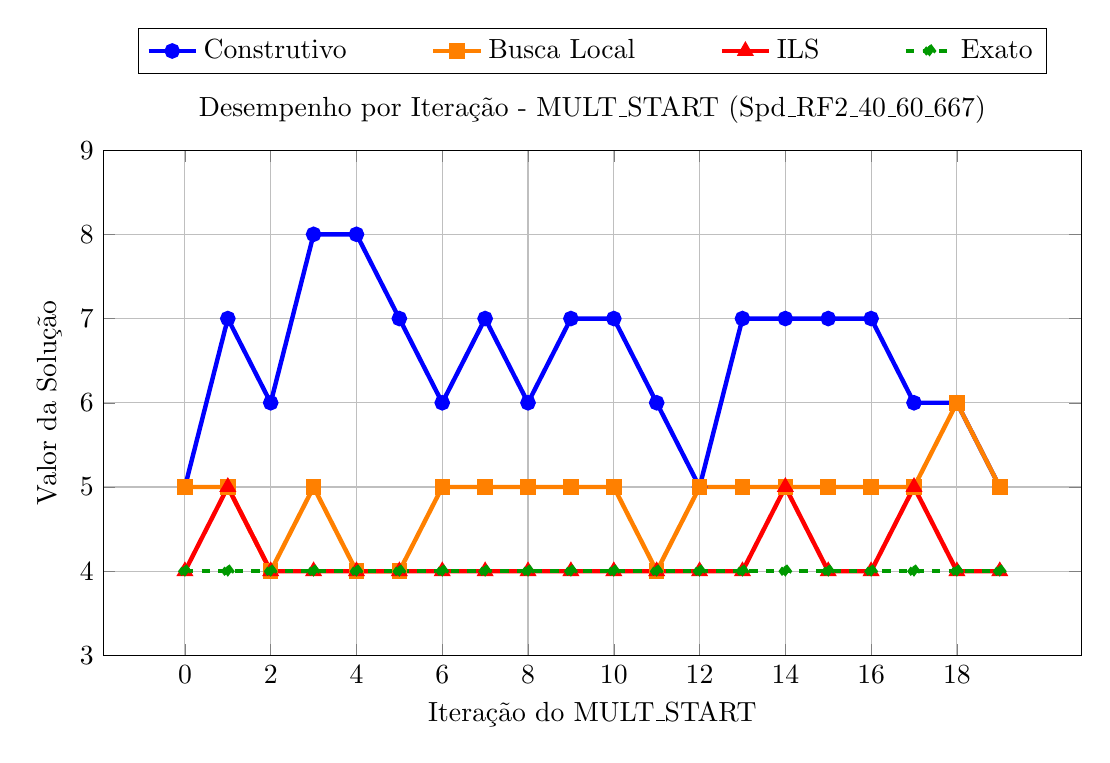
\begin{tikzpicture}
\begin{axis}[
    title={Desempenho por Iteração - MULT\_START (Spd\_RF2\_40\_60\_667)},
    xlabel={Iteração do MULT\_START},
    ylabel={Valor da Solução},
    grid=major,
    ymin=3, ymax=9,
    xtick={0,2,4,6,8,10,12,14,16,18},
    width=14cm,
    height=8cm,
    every axis plot/.append style={ultra thick},
    legend style={
        at={(0.5,1.15)},
        anchor=south,
        legend columns=-1,
        /tikz/every even column/.append style={column sep=1cm}
    }
]

% Construtivo
\addplot[color=blue, mark=*] coordinates {
(0,5) (1,7) (2,6) (3,8) (4,8) (5,7) (6,6) (7,7) (8,6) (9,7)
(10,7) (11,6) (12,5) (13,7) (14,7) (15,7) (16,7) (17,6) (18,6) (19,5)
};
\addlegendentry{Construtivo}

% Busca Local
\addplot[color=orange, mark=square*] coordinates {
(0,5) (1,5) (2,4) (3,5) (4,4) (5,4) (6,5) (7,5) (8,5) (9,5)
(10,5) (11,4) (12,5) (13,5) (14,5) (15,5) (16,5) (17,5) (18,6) (19,5)
};
\addlegendentry{Busca Local}

% ILS
\addplot[color=red, mark=triangle*] coordinates {
(0,4) (1,5) (2,4) (3,4) (4,4) (5,4) (6,4) (7,4) (8,4) (9,4)
(10,4) (11,4) (12,4) (13,4) (14,5) (15,4) (16,4) (17,5) (18,4) (19,4)
};
\addlegendentry{ILS}

% Exato
\addplot[color=green!60!black, mark=diamond*, dashed] coordinates {
(0,4) (1,4) (2,4) (3,4) (4,4) (5,4) (6,4) (7,4) (8,4) (9,4)
(10,4) (11,4) (12,4) (13,4) (14,4) (15,4) (16,4) (17,4) (18,4) (19,4)
};
\addlegendentry{Exato}

\end{axis}

\end{tikzpicture}

\vspace{0.5em}
\end{center}

\begin{center}
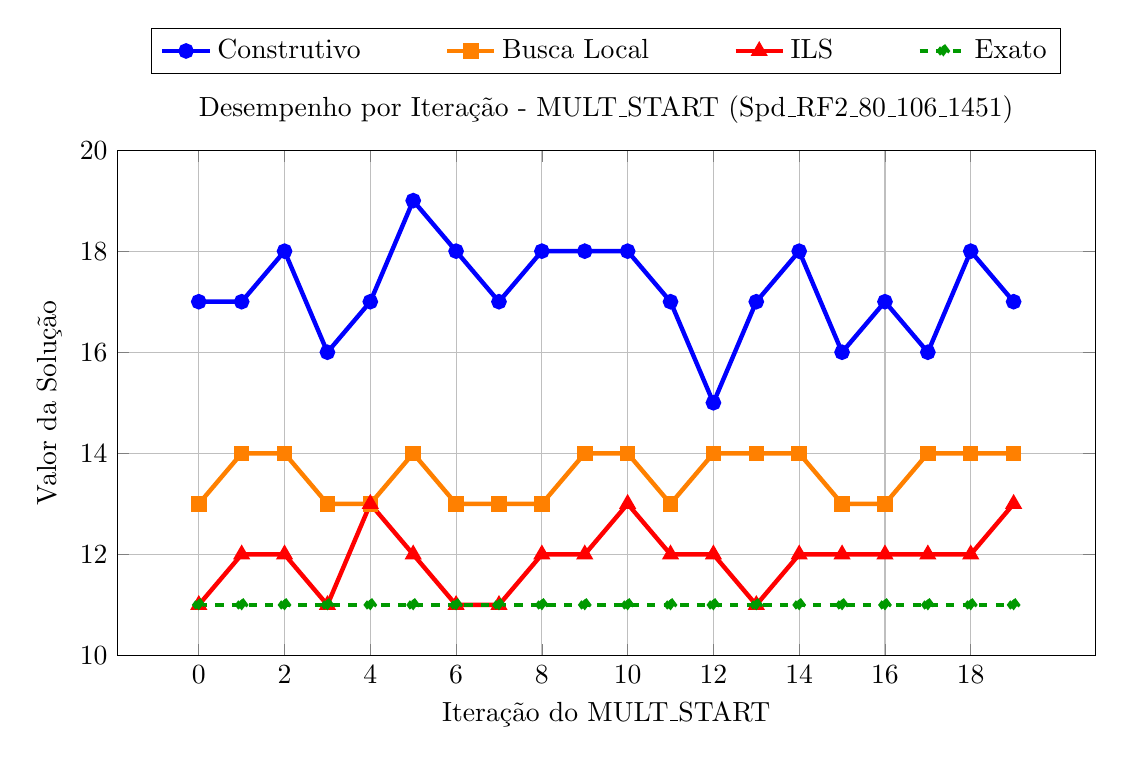
\begin{tikzpicture}
\begin{axis}[
    title={Desempenho por Iteração - MULT\_START (Spd\_RF2\_80\_106\_1451)},
    xlabel={Iteração do MULT\_START},
    ylabel={Valor da Solução},
    grid=major,
    ymin=10, ymax=20,
    xtick={0,2,4,6,8,10,12,14,16,18},
    width=14cm,
    height=8cm,
    every axis plot/.append style={ultra thick},
    legend style={
        at={(0.5,1.15)},
        anchor=south,
        legend columns=-1,
        /tikz/every even column/.append style={column sep=1cm}
    }
]

% Construtivo
\addplot[color=blue, mark=*] coordinates {
(0,17) (1,17) (2,18) (3,16) (4,17) (5,19) (6,18) (7,17) (8,18) (9,18)
(10,18) (11,17) (12,15) (13,17) (14,18) (15,16) (16,17) (17,16) (18,18) (19,17)
};
\addlegendentry{Construtivo}

% Busca Local
\addplot[color=orange, mark=square*] coordinates {
(0,13) (1,14) (2,14) (3,13) (4,13) (5,14) (6,13) (7,13) (8,13) (9,14)
(10,14) (11,13) (12,14) (13,14) (14,14) (15,13) (16,13) (17,14) (18,14) (19,14)
};
\addlegendentry{Busca Local}

% ILS
\addplot[color=red, mark=triangle*] coordinates {
(0,11) (1,12) (2,12) (3,11) (4,13) (5,12) (6,11) (7,11) (8,12) (9,12)
(10,13) (11,12) (12,12) (13,11) (14,12) (15,12) (16,12) (17,12) (18,12) (19,13)
};
\addlegendentry{ILS}

% Exato
\addplot[color=green!60!black, mark=diamond*, dashed] coordinates {
(0,11) (1,11) (2,11) (3,11) (4,11) (5,11) (6,11) (7,11) (8,11) (9,11)
(10,11) (11,11) (12,11) (13,11) (14,11) (15,11) (16,11) (17,11) (18,11) (19,11)
};
\addlegendentry{Exato}

\end{axis}
\end{tikzpicture}
\end{center}

\begin{center}
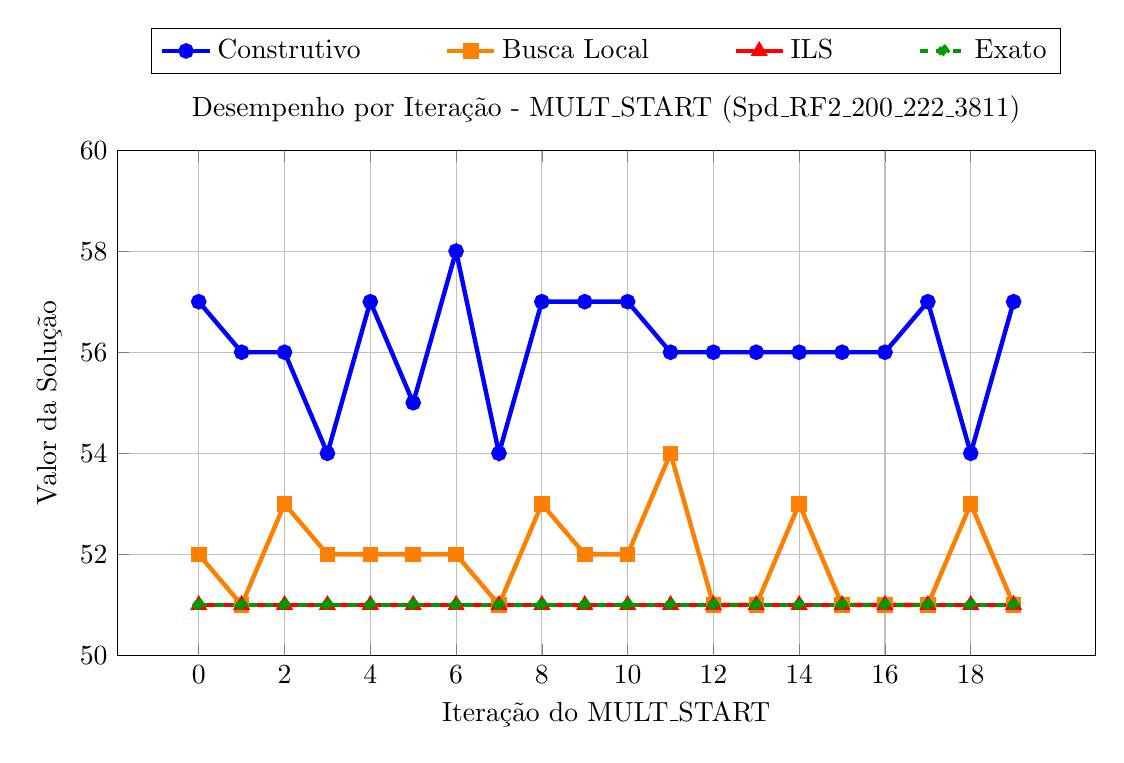
\begin{tikzpicture}
\begin{axis}[
    title={Desempenho por Iteração - MULT\_START (Spd\_RF2\_200\_222\_3811)},
    xlabel={Iteração do MULT\_START},
    ylabel={Valor da Solução},
    grid=major,
    ymin=50, ymax=60,
    xtick={0,2,4,6,8,10,12,14,16,18},
    width=14cm,
    height=8cm,
    every axis plot/.append style={ultra thick},
    legend style={
        at={(0.5,1.15)},
        anchor=south,
        legend columns=-1,
        /tikz/every even column/.append style={column sep=1cm}
    }
]

% Construtivo
\addplot[color=blue, mark=*] coordinates {
(0,57) (1,56) (2,56) (3,54) (4,57) (5,55) (6,58) (7,54) (8,57) (9,57)
(10,57) (11,56) (12,56) (13,56) (14,56) (15,56) (16,56) (17,57) (18,54) (19,57)
};
\addlegendentry{Construtivo}

% Busca Local
\addplot[color=orange, mark=square*] coordinates {
(0,52) (1,51) (2,53) (3,52) (4,52) (5,52) (6,52) (7,51) (8,53) (9,52)
(10,52) (11,54) (12,51) (13,51) (14,53) (15,51) (16,51) (17,51) (18,53) (19,51)
};
\addlegendentry{Busca Local}

% ILS
\addplot[color=red, mark=triangle*] coordinates {
(0,51) (1,51) (2,51) (3,51) (4,51) (5,51) (6,51) (7,51) (8,51) (9,51)
(10,51) (11,51) (12,51) (13,51) (14,51) (15,51) (16,51) (17,51) (18,51) (19,51)
};
\addlegendentry{ILS}

% Exato
\addplot[color=green!60!black, mark=diamond*, dashed] coordinates {
(0,51) (1,51) (2,51) (3,51) (4,51) (5,51) (6,51) (7,51) (8,51) (9,51)
(10,51) (11,51) (12,51) (13,51) (14,51) (15,51) (16,51) (17,51) (18,51) (19,51)
};
\addlegendentry{Exato}

\end{axis}
\end{tikzpicture}
\end{center}


\begin{center}
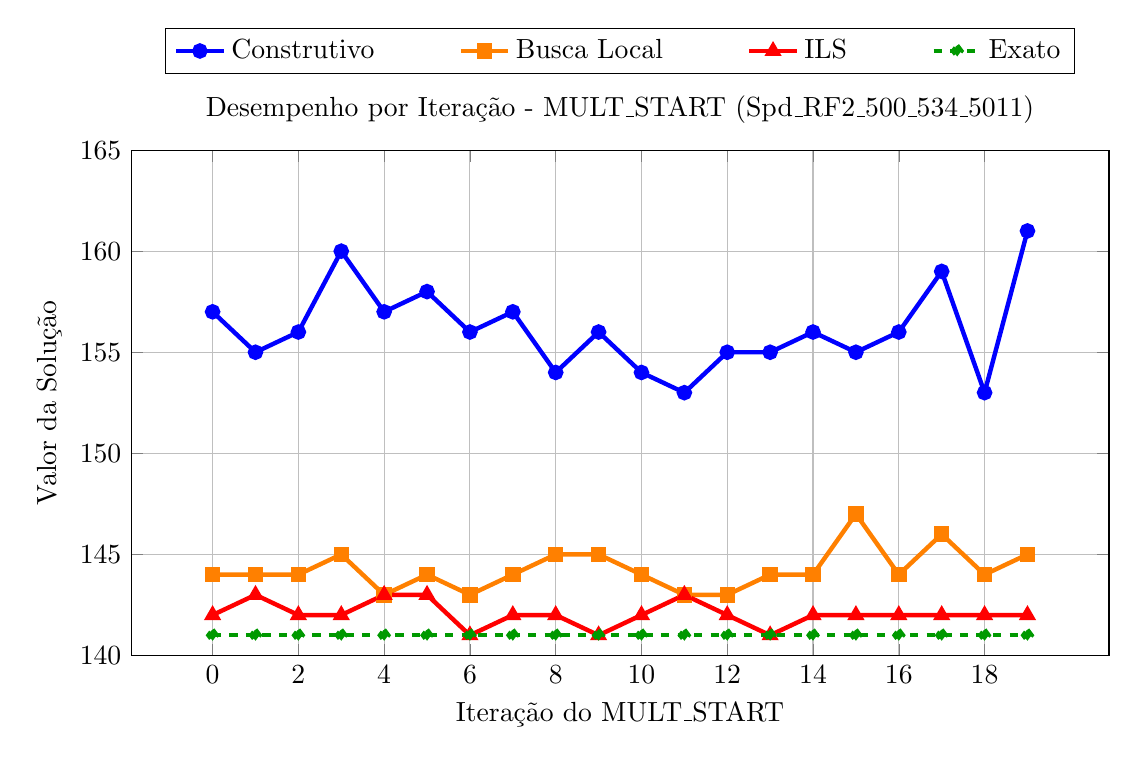
\begin{tikzpicture}
\begin{axis}[
    title={Desempenho por Iteração - MULT\_START (Spd\_RF2\_500\_534\_5011)},
    xlabel={Iteração do MULT\_START},
    ylabel={Valor da Solução},
    grid=major,
    ymin=140, ymax=165,
    xtick={0,2,4,6,8,10,12,14,16,18},
    width=14cm,
    height=8cm,
    every axis plot/.append style={ultra thick},
    legend style={
        at={(0.5,1.15)},
        anchor=south,
        legend columns=-1,
        /tikz/every even column/.append style={column sep=1cm}
    }
]

% Construtivo
\addplot[color=blue, mark=*] coordinates {
(0,157) (1,155) (2,156) (3,160) (4,157) (5,158) (6,156) (7,157) (8,154) (9,156)
(10,154) (11,153) (12,155) (13,155) (14,156) (15,155) (16,156) (17,159) (18,153) (19,161)
};
\addlegendentry{Construtivo}

% Busca Local
\addplot[color=orange, mark=square*] coordinates {
(0,144) (1,144) (2,144) (3,145) (4,143) (5,144) (6,143) (7,144) (8,145) (9,145)
(10,144) (11,143) (12,143) (13,144) (14,144) (15,147) (16,144) (17,146) (18,144) (19,145)
};
\addlegendentry{Busca Local}

% ILS
\addplot[color=red, mark=triangle*] coordinates {
(0,142) (1,143) (2,142) (3,142) (4,143) (5,143) (6,141) (7,142) (8,142) (9,141)
(10,142) (11,143) (12,142) (13,141) (14,142) (15,142) (16,142) (17,142) (18,142) (19,142)
};
\addlegendentry{ILS}

% Exato
\addplot[color=green!60!black, mark=diamond*, dashed] coordinates {
(0,141) (1,141) (2,141) (3,141) (4,141) (5,141) (6,141) (7,141) (8,141) (9,141)
(10,141) (11,141) (12,141) (13,141) (14,141) (15,141) (16,141) (17,141) (18,141) (19,141)
};
\addlegendentry{Exato}

\end{axis}
\end{tikzpicture}
\end{center}


\begin{center}
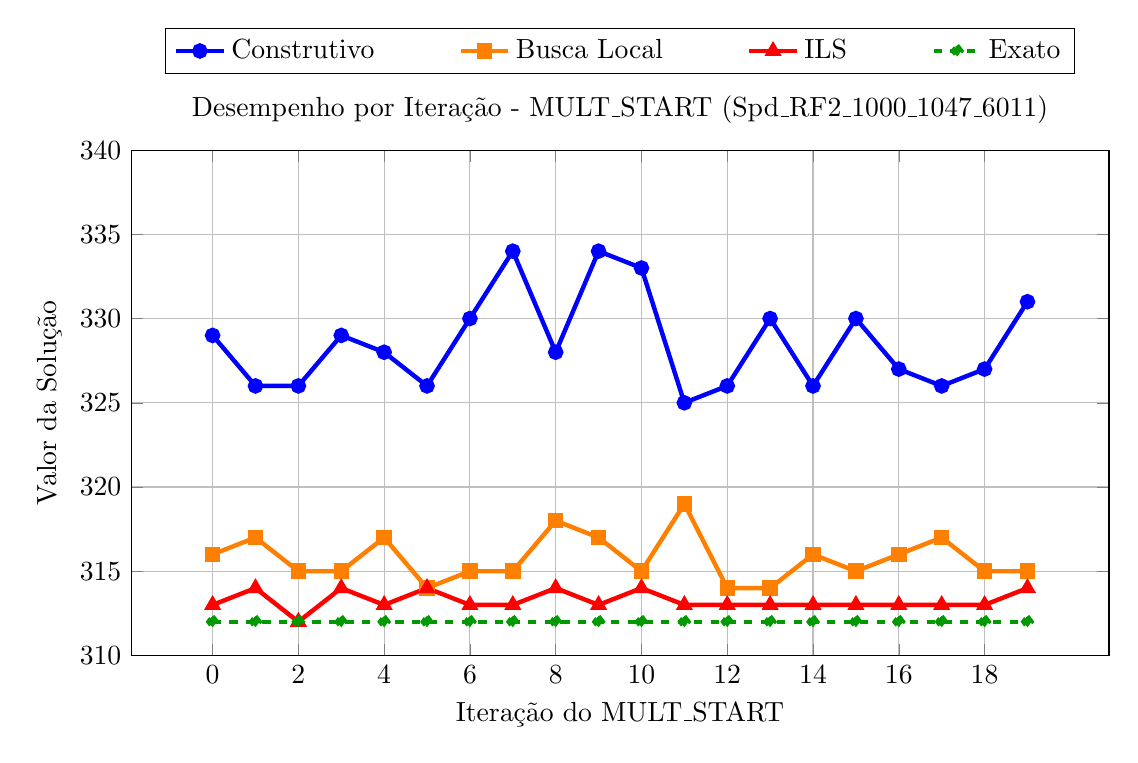
\begin{tikzpicture}
\begin{axis}[
    title={Desempenho por Iteração - MULT\_START (Spd\_RF2\_1000\_1047\_6011)},
    xlabel={Iteração do MULT\_START},
    ylabel={Valor da Solução},
    grid=major,
    ymin=310, ymax=340,
    xtick={0,2,4,6,8,10,12,14,16,18},
    width=14cm,
    height=8cm,
    every axis plot/.append style={ultra thick},
    legend style={
        at={(0.5,1.15)},
        anchor=south,
        legend columns=-1,
        /tikz/every even column/.append style={column sep=1cm}
    }
]

% Construtivo
\addplot[color=blue, mark=*] coordinates {
(0,329) (1,326) (2,326) (3,329) (4,328) (5,326) (6,330) (7,334) (8,328) (9,334)
(10,333) (11,325) (12,326) (13,330) (14,326) (15,330) (16,327) (17,326) (18,327) (19,331)
};
\addlegendentry{Construtivo}

% Busca Local
\addplot[color=orange, mark=square*] coordinates {
(0,316) (1,317) (2,315) (3,315) (4,317) (5,314) (6,315) (7,315) (8,318) (9,317)
(10,315) (11,319) (12,314) (13,314) (14,316) (15,315) (16,316) (17,317) (18,315) (19,315)
};
\addlegendentry{Busca Local}

% ILS
\addplot[color=red, mark=triangle*] coordinates {
(0,313) (1,314) (2,312) (3,314) (4,313) (5,314) (6,313) (7,313) (8,314) (9,313)
(10,314) (11,313) (12,313) (13,313) (14,313) (15,313) (16,313) (17,313) (18,313) (19,314)
};
\addlegendentry{ILS}

% Exato
\addplot[color=green!60!black, mark=diamond*, dashed] coordinates {
(0,312) (1,312) (2,312) (3,312) (4,312) (5,312) (6,312) (7,312) (8,312) (9,312)
(10,312) (11,312) (12,312) (13,312) (14,312) (15,312) (16,312) (17,312) (18,312) (19,312)
};
\addlegendentry{Exato}

\end{axis}
\end{tikzpicture}
\end{center}